\chapter{Design and implementation}\label{chapter:design}

In this chapter we delve into the design and the implementation details of
\emph{iptables-to-sefl}, the tool we built to generate SEFL models from
iptables configurations.

We start by presenting the template we use to build models for iptables-enabled
devices.  We increase its complexity and the amount of details as we gradually
introduce features supported in the finalized project.  Following that, we
cover most of the implementation-related decisions that are particularly
distinctive to our tool.  We sum up this chapter with an overview of the
limitations that come up along the way.


\section{Towards a model}

Building a SEFL model which can then be verified by SymNet is as simple as
providing two Map data structures, as discussed in
\labelindexref{Section}{sec:symnet-sefl}:
\begin{enumerate}[a)]
  \item the first one, from \emph{source} ports to \emph{destination} ports; it
    implicitly defines a directed graph which is our formal way of defining
    networks.
  \item the other one, from \emph{ports} (i.e. nodes in this graph) to SEFL
    instructions; this one captures the actual behaviour of each network
    element.
\end{enumerate}

The goal of this chapter is to show how we provide these Maps starting from a
deployment of iptables rules, in such a way that once fed into SymNet, the
verified behaviour is that of an iptables-enabled device.  To do so, in this
section we start by describing the high-level idea of our model as well as the
underlying algorithms that we use.

\bigskip

To ease the bootstrapping of our modelling process, we notice that packet
processing in netfilter is built around the routing decision.  To be more
precise, in \labelindexref{Figure}{fig:iptables-organization} from the previous
chapter there are three points in the processing stack where the routing table
is consulted.  Moreover, a routing decision was the only feature of the simple
router model we introduced in \labelindexref{Section}{sub-sec:building-models}.
Well-known software engineering practices tell us that we should reuse existing
functionality as long as it makes sense to do so.  In our scenario, it does.

Thus, in the first iteration towards our end goal of reaching an iptables model
from a router model we separate the only routing decision featured in
\labelindexref{Figure}{fig:router-model} into three different routing
decisions, as shown in \labelindexref{Figure}{fig:iptables-1}.

\begin{figure}[h]
  \centering
  \captionsetup{justification=centering}
  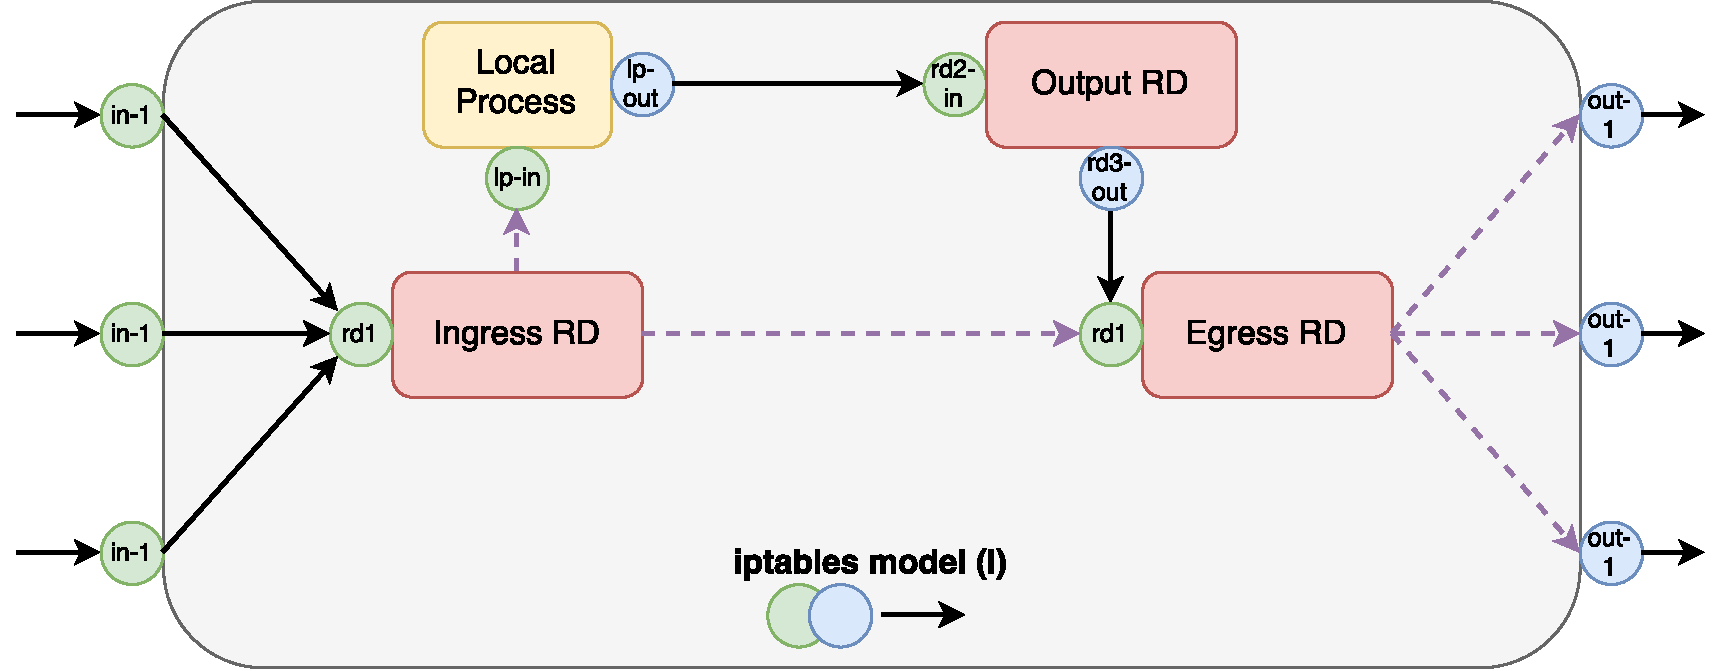
\includegraphics[scale=0.5]{src/img/iptables-1}
  \caption[iptables model (I): Separated routing decisions.]{iptables model
  (I): Separated routing decisions.  Straight arrows correspond to directed
  edges in our network model, while dotted-arrows correspond to possible
  \emph{Forward} instructions directing traffic on those paths. Note that it is
  important to assign unique port names because there are no name scopes;
  implementation-wise, this is achieved by prefixing the \emph{role} of the
  port (e.g.  \emph{in}, \emph{out}) by the unique name of the \emph{virtual
  device} it belongs to.}
  \label{fig:iptables-1}
\end{figure}

Note that we \emph{specialized} each one of the three new routing decisions:
\begin{itemize}
  \item \textbf{ingress} routing decision: for traffic that \textbf{enters}
    this device
  \item \textbf{egress} routing decision: for traffic that \textbf{exits} this
    device
  \item \textbf{output} (sometimes \emph{local}) routing decision: for traffic
    that is \textbf{generated by} this device
\end{itemize}

Another thing that might not be obvious at first is that the behaviour of two
out of three of them has changed.  It is easier to see this if we focus on the
one for locally generated packets.  We notice that its single output port is
connected to the input port of the \emph{egress} one, which means that all
packets that enter it will follow that path.  Thus, it does not capture the
usual routing decision behaviour which simply forwards packets to output ports
based on some logic (i.e. destination IP and routing table).  The same applies
to \emph{ingress} which only partitions packets based on whether they should be
delivered locally or not.  It turns out that this new behaviour is essential to
iptables, to enable matching against the output interface in the
FORWARD/POSTROUTING chains, or to allow redirecting traffic in nat/OUTPUT. It
is usually implemented by storing the decision (output port) instead of
forwarding packets based on it.

As simple as this step might be, it still corresponds to a valid iptables
configuration: the \emph{void} one.  This is a valuable remark because it
allows us to validate future, more complex versions of the model by comparing
their output when all chains/tables are empty to that of this
\emph{featureless} one (a form of \textbf{regression testing}).

\bigskip

To advance one more step in our attempt to reach a model of an iptables-enabled
device, let us observe the similarity between
\labelindexref{Figure}{fig:iptables-1} and
\labelindexref{Figure}{fig:iptables-organization} from
\labelindexref{Chapter}{chapter:background}.  It seems that all we need to do
in order to make them be truly alike is to add some \emph{virtual devices} to
model chain traversal. The resulting schema is shown in
\labelindexref{Figure}{fig:iptables-2}.

\begin{figure}[h]
  \centering
  \captionsetup{justification=centering}
  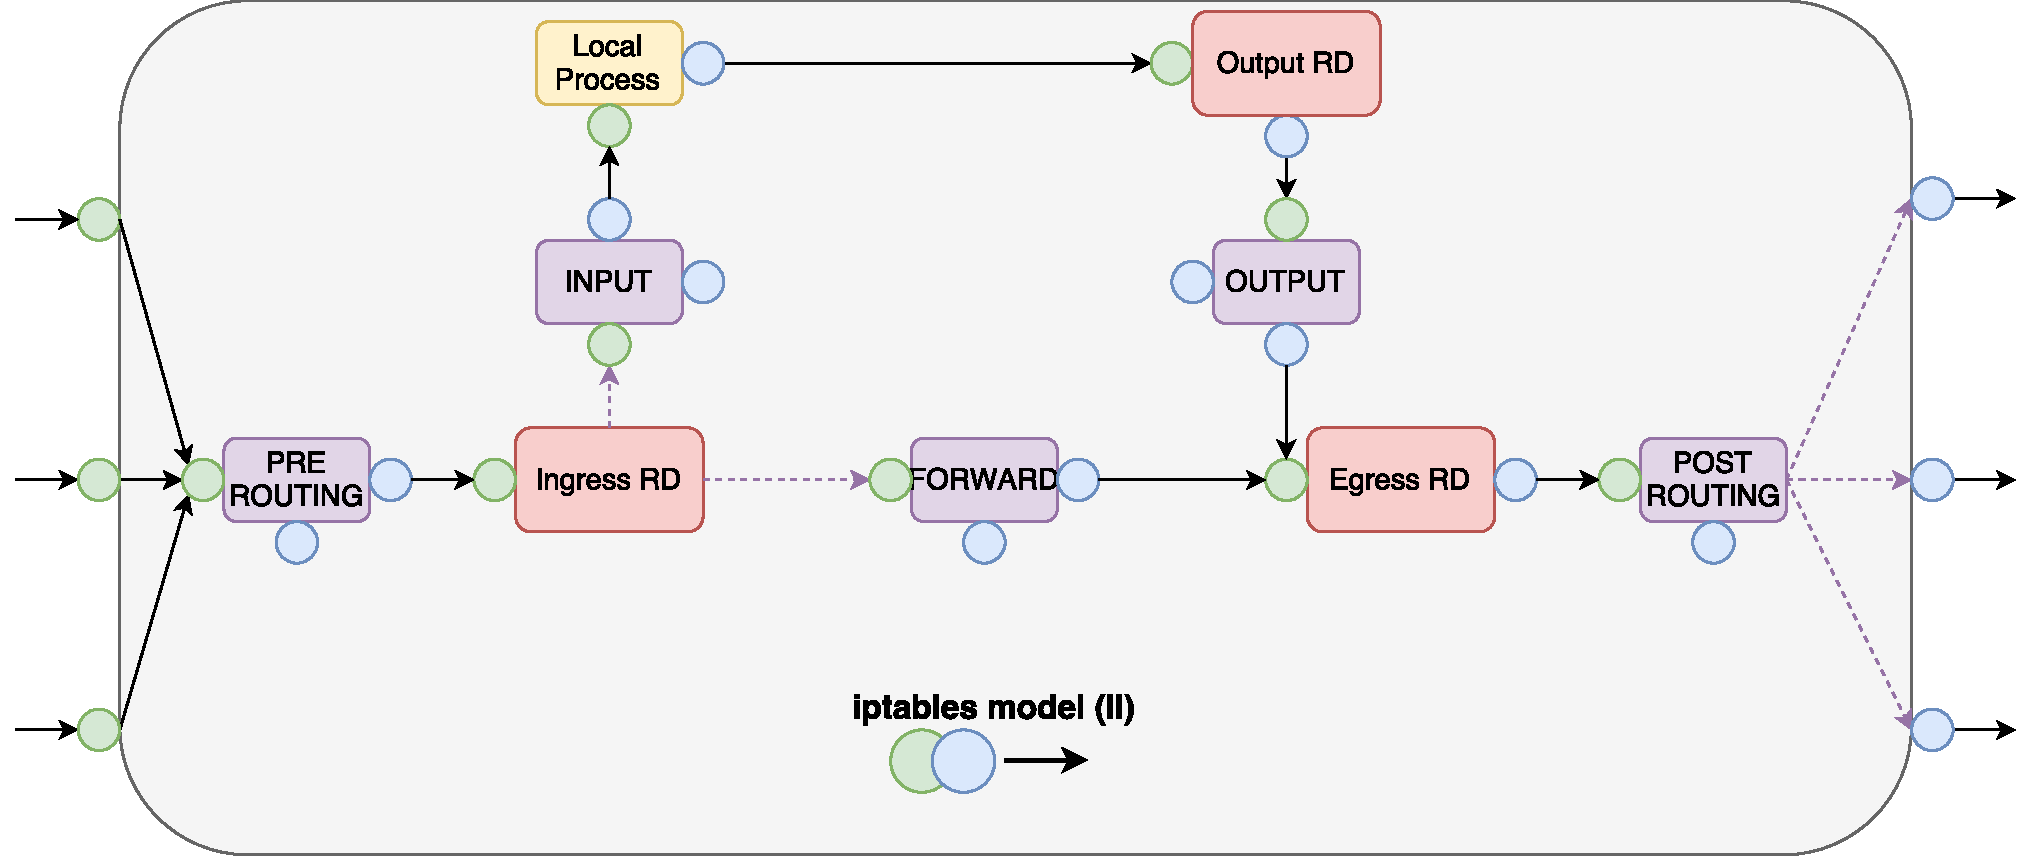
\includegraphics[scale=0.45]{src/img/iptables-2}
  \caption[iptables model (II): Incorporated chain virtual devices.]{iptables
  model (II): Incorporated chain virtual devices.  The purple squares are
  Iptables Virtual Devices (IVDs) and they abstract chain traversal logic.}
  \label{fig:iptables-2}
\end{figure}

The new virtual devices are called \textbf{Iptables Virtual Devices}
(IVD)\abbrev{IVD}{Iptables Virtual Devices} and have the distinctive feature
that always have one input port and two output ports: an output port
corresponding to \emph{accepting} packets, whether modified or not, and another
one for \emph{dropping} packets, which is especially useful when modelling the
filter table.  In \labelindexref{Figure}{fig:iptables-2}, the former
corresponds to the output ports (blue circles) of IVDs (purple squares) which
are linked to the next virtual device in the processing stack.  On the other
hand, the \emph{dropping} ports are not connected to any other ports and have a
SEFL \hltexttt{Fail} instruction associated with them.

So what does this new augmented model buy us?  Firstly, as already mentioned,
it is closer (at least from a high-level perspective for now) to the internal
organization of iptables.  Secondly, it further separates the actual iptables
logic to be modelled on a per-chain basis.  In fact, this can be further
divided by acknowledging that each chain IVD, as it represented here, is a
sequence of concrete (per table) chain traversals; for instance, there are 3
tables that might define rules in the PREROUTING chain: raw, mangle, nat.
Therefore, we can improve our model by splitting each chain IVD as shown in
\labelindexref{Figure}{fig:iptables-2-composition}.

\begin{figure}[h]
  \centering
  \captionsetup{justification=centering}
  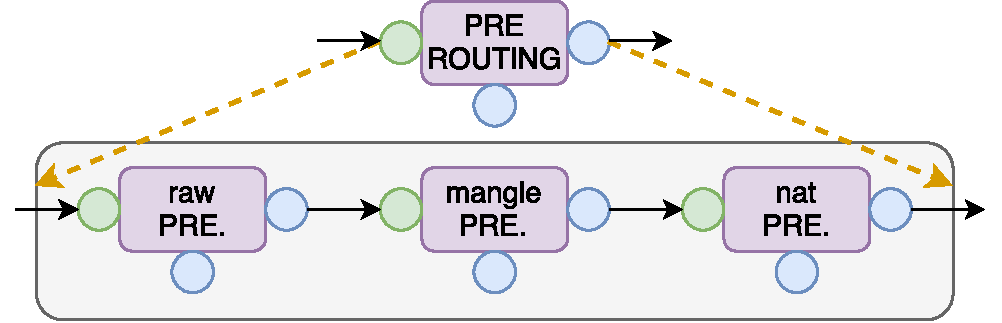
\includegraphics[scale=0.5]{src/img/iptables-2-composition}
  \caption[Concrete (per-table chains) make up individual chain IVDs.]{Concrete
  (per-table chains) make up individual chain IVDs.}
  \label{fig:iptables-2-composition}
\end{figure}

Thus, we can assert that we reduced our problem of modelling an
iptables-enabled device to that of implementing (in SEFL) the traversal of a
chain of rules. \labelindexref{Algorithm}{algo:chain-traversal} captures the
naive but straightforward way of doing that:

\begin{algorithm}[H]
  \SetKwInOut{Inputs}{inputs}
  \SetKwInOut{Output}{output}
  \SetKwProg{TraverseChain}{TraverseChain}{}{}

  \TraverseChain{$(C, P)$}{
    \Inputs{A chain $C$ and a packet $P$}
    \Output{The target $T$ to jump to}

    \ForEach{rule $r \in$ C.rules}{
      \If{$m(p)$ is true $\forall m \in$ r.matches}{
        \textbf{return} $r.target$
      }
    }
    \textbf{return} $C.policy$
  }
  \caption[Traversing a chain.]{Traversing a chain. A chain aggregates a list
  of \emph{rules} and a \emph{default target} (i.e. policy). A rule contains a
  list of \emph{matches} and a \emph{target}.}
  \label{algo:chain-traversal}
\end{algorithm}

It is possible to express this algorithm in SEFL.  However, there are two
problems with it:
\begin{itemize}
  \item It \textbf{ignores} a couple of essential features in iptables (e.g.
    jumping to user-defined chains).  Thus,
    \labelindexref{Figure}{fig:iptables-2}, even though correct in terms of the
    abstractions it makes, it hides a couple of rather involved functionality.
  \item It could be inefficient due to many \hltexttt{if/then/else} statements
    that result.  It is worth reiterating here that SEFL and SymNet do not give
    outstanding performance results by default; they require well crafted
    models.
\end{itemize}

We tackle the former in the next couple of sections.

\subsection{User-defined chains}
\todo{explain WHY they complicate the simple model in the previous section.
explain that our final model reflects their exact semantics}
\todo{what is an Iptables Virtual Device (IVD); what is a Chain IVD; cover in
detail all components of a Chain IVD: input dispatcher, contiguous IVDs, output
dispatchers}

\subsection{Network Address Translation}
\todo{start with all kinds of NAT supported? SNAT, DNAT, MASQUERADE (mention
that it is essentially SNAT, since we model data plane only), REDIRECT}
\todo{WHY we treat NAT separately? mention the fact that for each flow, NAT
tables are consulted once only, and then the applied rule is automatically
re-applied; this means that custom logic that SKIPS the table has to be added;
show how this changes the model we reached in the previous section; add the
Chain IVD Initializer components.}
\todo{besides that, reply-packets have to be reverse-NAT'ed}

\subsection{Connection tracking}
\todo{show how we introduce a new \emph{virtual device} that implements the
connection tracking logic. mention that it is currently limited, only NEW to
ESTABLISHED is handled; explain how it works, more precisely; also mention that
a great limitation is discussed in
\labelindexref{Section}{sub-sec:related-state}.}

\bigskip
\todo{conclude by saying that it finalizes the current state of our model,
which is quite involved compared to the initial one we devised at the beginning
of this section.}


\section{Implementation}\label{sec:implementation}
\todo{Could also mention the size of the project; 4k + 4k, "out of tree"
(SymNet); not really "test-driven", but more like "tested"}
\todo{this chapter shows how some of the things discussed in the previous
section are implemented;}
\todo{add implementation-detailed diagrams of the 'iptelement' hierarchy as
well as of the 'virtualdevice' hierarchy; mention composite approach, etc.}
\todo{(inspired by todo 1 above) Discuss what the interface with SymNet is. --
these parts (Instruction/:==:, etc) will be added to a separate "api" package,
to be easily accessed by other models and for better code organization.}
\todo{Before delving into the next subsections, could also mention code
structure, 3 main directories (core, extensions - one directory for each
extension -, virtdev), the driver in the root}

\subsection{Parsing}
\todo{talk about parsing, table parsing, chain parsing, ParsingContext, rule
parsing, match/target parsing, their extensions, how they are extended, etc}
\todo{for rule parsing, mention the functionality behind the 'match extension
activation', flag -m or --match}
\todo{Monadic, Parsec, functional, haskell etc}

\subsection{Validation}
\todo{WHY it is needed; say that it is analogous to semantic analysis in
compilers}
\todo{use cases: unordered chains (needed), port range validity, certain chains
in certain tables, certain rules in certain tables/chains, etc}
\todo{how it works, validate() function, validateIf variant, ValidationContext}

\subsection{Code generation}
\todo{SeflGenOptions trait, the variant for match extensions and the one for
target extensions}


\section{Extensions}
\todo{is this section still needed? maybe add some examples in the previous
sections, rather than adding another one}
\subsection{TCP and UDP}
\subsection{MARK and CONNMARK}


\section{Limitations}
\todo{We build precise models, as far as our toolset (SymNet, SEFL) permits.
However, there are certain limitations which are discussed next.}

\subsection{The local process}
\todo{say that we are not interested in modelling the local process, as a
correct, or at least close to one, model of that would be the kernel itself,
plus application specific logic.}
\todo{however, one trick we do to allow 'simulation' of traffic generated by
some applications is to expose its output port from figure XX. this permits
starting symbolic execution by injecting a symbolic packet on that port and see
what happens, etc.}

\subsection{The RELATED connection state}\label{sub-sec:related-state}
\todo{say again what its purpose should be; give an use-case}
\todo{Inherent limitation caused by the independence between different flows.}
